% Report for the AirPLAi CV trial project: what was built, what it scored, what broke.
% Build: make report   (pdflatex twice, for the table of contents)
\documentclass[10pt,a4paper]{article}

\usepackage[T1]{fontenc}
\usepackage[utf8]{inputenc}
\usepackage{charter}
\usepackage{microtype}
\usepackage[margin=18mm,top=16mm,bottom=18mm]{geometry}
\usepackage{booktabs}
\usepackage{tabularx}
\usepackage{xltabular}
\usepackage{array}
\usepackage[dvipsnames]{xcolor}
\usepackage{enumitem}
\usepackage{titlesec}
\usepackage[hang,flushmargin]{footmisc}
\makeatletter\renewcommand{\@makefntext}[1]{\raggedright\noindent\@makefnmark\,#1}\makeatother
\usepackage[font=small,labelfont=bf,skip=6pt]{caption}
\usepackage{float}
\usepackage{graphicx}
\graphicspath{{docs/}{./}}
\usepackage[colorlinks=true,linkcolor=Sepia,urlcolor=Sepia,citecolor=Sepia]{hyperref}

\definecolor{slate}{RGB}{48,56,68}
\definecolor{accent}{RGB}{198,102,36}
\definecolor{mute}{RGB}{120,128,138}

\titleformat{\section}{\large\bfseries\color{slate}}{\thesection}{0.7em}{}
\titleformat{\subsection}{\normalsize\bfseries\color{slate}}{\thesubsection}{0.6em}{}
\titlespacing*{\section}{0pt}{10pt}{4pt}
\titlespacing*{\subsection}{0pt}{7pt}{2pt}

\setlist[itemize]{leftmargin=1.2em,itemsep=2pt,topsep=3pt}
\setlength{\parskip}{2pt}
\renewcommand{\arraystretch}{1.05}
\setlength{\LTpre}{6pt}\setlength{\LTpost}{6pt}

\newcolumntype{L}[1]{>{\raggedright\arraybackslash}p{#1}}
\newcolumntype{R}[1]{>{\raggedleft\arraybackslash}p{#1}}
\newcommand{\design}[1]{%
  \par\smallskip\noindent
  {\color{accent!88!black}\small\textbf{$\triangleright$ As designed.} \textit{#1}}\par\smallskip}

\title{\vspace{-16mm}\bfseries\color{slate}Dodgeball Throw-Attempt Detection\\[1mm]
       \large\mdseries Report}
\author{Gary Ferguson}
\date{\vspace{-2mm}27 August 2026}

\begin{document}
\maketitle
\thispagestyle{empty}

\noindent
\begin{minipage}{\textwidth}
\small\color{slate}
\rule{\textwidth}{0.4pt}\\[3pt]
\textbf{What this is.} The report on the build: what was made, what it scored, where it
broke, and which parts of the design the measurements overturned. The design is
\texttt{docs/design.pdf}; the shipped design of each stage is in
\texttt{docs/architecture/}. Every number here is reproduced by the commands in
\S\ref{sec:repro} from a clean checkout.

Times are clip time, m:ss from the start of the 3.5-minute cut. Decisions the build
overturned are marked \textcolor{accent!88!black}{$\triangleright$} with the design's
version beside the built one.\\[2pt]
\rule{\textwidth}{0.4pt}
\end{minipage}

\vspace{1mm}
{\small\setcounter{tocdepth}{2}\tableofcontents}
\clearpage

%=====================================================================
\section{What was built}
\label{sec:built}

The footage is the second half of the 2014 World Dodgeball Championship men's final,
Canada against USA, one fixed elevated end-on camera for the whole half at 1920$\times$1080
and 25\,fps.\footnote{World Dodgeball Federation, \emph{2014 World Dodgeball
Championship, Men's Final: Canada v USA} [video], YouTube,
$<$\url{https://www.youtube.com/watch?v=Spu6OlAZHUo}$>$, accessed 27 August 2026.} The
evaluation clip is 6:00 to 9:30 of that half: one complete set, from the opening rush to
the next, 3.5 minutes, 5,250 frames. USA is the far team and Canada the near one in every
table below. The full half, 23 minutes and eight sets, was run unlabelled for
\S\ref{sec:scale}.

The pipeline shipped as eleven stages, each a script writing one file that the next reads.

{\footnotesize
\begin{xltabular}{\textwidth}{L{26mm} X L{40mm}}
\toprule
\textbf{Stage} & \textbf{As shipped} & \textbf{Against the design}\\
\midrule
Court fit & Median background plate, HSV line extraction, homography to metres, checked against markings not used in the fit & As designed\\
Pose & YOLO11x-pose\footnote{G.\ Jocher, J.\ Qiu and A.\ Chaurasia, \emph{Ultralytics YOLO} (version 8.4), software, 2024, $<$\url{https://github.com/ultralytics/ultralytics}$>$, accessed 27 August 2026.} at 1920\,px, every frame, once per clip, single precision & As designed; half precision benchmarked, not run (\S\ref{sec:compute})\\
Set start & Balls laid on the centre line arm a window, a whistle inside it is the start, both teams breaking for the balls confirms it & As designed\\
Roster & ByteTrack\footnote{Y.\ Zhang, P.\ Sun, Y.\ Jiang, D.\ Yu, F.\ Weng, Z.\ Yuan, P.\ Luo, W.\ Liu and X.\ Wang, `ByteTrack: Multi-Object Tracking by Associating Every Detection Box', in \emph{Computer Vision -- ECCV 2022}, Lecture Notes in Computer Science 13682 (Cham: Springer, 2022), pp.\ 1--21.} fragments joined by jersey number (EasyOCR\footnote{JaidedAI, \emph{EasyOCR} (version 1.7), software, $<$\url{https://github.com/JaidedAI/EasyOCR}$>$, accessed 27 August 2026; its detector is Y.\ Baek, B.\ Lee, D.\ Han, S.\ Yun and H.\ Lee, `Character Region Awareness for Text Detection', in \emph{2019 IEEE/CVF Conference on Computer Vision and Pattern Recognition} (Long Beach, 2019), pp.\ 9357--9366.} on the best crops) and side; a player is whoever is in play during the set's core & As designed, plus the in-play test: a referee's stripes and USA's black print read alike to the kit rule\\
Set end & One side down to a single player, then the court flooding with bodies & Designed as ``the last elimination''; built as a state test because the elimination itself is what the outcome stage is trying to find\\
Candidates & Wrist speed against the torso, normalised by depth; wind-up past the shoulder line; every window a duration converted at the clip's frame rate & As designed\\
Release gate & Ball as colour at the wrists before the peak, then a chain of ball-sized blobs seen leaving the hand & As designed; the pose features for follow-through were tested and dropped (\S\ref{sub:signals})\\
Destination & Contact with a player's box where the chain reaches one, otherwise the chain's first direction in the image against the centre line & Changed (\S\ref{sub:dest})\\
Rebound & SAM~2\footnote{N.\ Ravi, V.\ Gabeur, Y.-T.\ Hu, R.\ Hu, C.\ Ryali, T.\ Ma, H.\ Khedr, R.\ R\"adle, C.\ Rolland, L.\ Gustafson, E.\ Mintun, J.\ Pan, K.\ V.\ Alwala, N.\ Carion, C.-Y.\ Wu, R.\ Girshick, P.\ Doll\'ar and C.\ Feichtenhofer, `SAM 2: Segment Anything in Images and Videos', arXiv:2408.00714, 2024.} seeded on the chain's last clean blob, following the ball to the player it reaches and through, on a crop that moves with it; reports whether the ball turned there & New stage (\S\ref{sub:outcome})\\
Outcome & A persistent step in a side's on-court count is a hit, or a catch if the other side gains one, attributed to the last throw at that side; the rebound splits two throws inside the lag and claims blocks & Changed (\S\ref{sub:outcome})\\
Evaluation & One score per level, error budget, stress, ablation, plus the set-up split of \S\ref{sec:scale} & As designed, plus the split\\
\bottomrule
\end{xltabular}}

Nothing was trained. The two contracts in the design held: every derived file records
the clip's SHA-256 and refuses another cut, and what is assumed about the venue (ball
colour window, court dimensions, kit colours) lives in \texttt{config/venue.toml} and
nowhere else.

%=====================================================================
\section{What changed from the design}
\label{sec:changed}

\subsection{Outcome from the count, the ball as witness}
\label{sub:outcome}

\design{The short post-release trajectory decides outcome; the on-court count checks it.}

The chain of ball blobs dies at the target's box. At 25\,fps and twenty pixels the frame
where the ball meets a player is the frame the contact and everything after it are against
the body, so a dodge and a hit looked the same to the chain, and the whistle sounded for
fakes too (\S\ref{sub:signals}). What was observable was that someone left. Only a throw
resolving moves the count, so the outcome was read from the game: a persistent step in a
side's on-court count is a hit, or a catch if the other side gains a player, attributed to
the last throw at that side inside the lag. That alone scored 13 of 22 outcomes right, and
its two blind spots were the ones the design had named as the biggest structural risk: two
throws at one side inside the lag, where recency picks the later one and scores two errors,
and blocks, which move no count and leave nothing in the state to see.

So the ball was brought back, to break ties rather than to judge. SAM~2 is seeded on the chain's last clean
blob and follows the ball to the player it reaches and through, on a crop that moves with
it. Contact is the box the ball \emph{turns} in rather than the first it enters, because a
ball passing beside a crouching player enters the box without touching them. On the clip a ball
that struck a player came back off them at 77--130$^\circ$; one that carried past turned
under 40$^\circ$; the threshold sits at 60$^\circ$. Where two throws compete for one
departure, the one whose ball turned takes it; a ball that turned and put nobody out was
blocked. That took the outcome to 18 of 22 (\S\ref{sec:wrong}). The threshold was set by
eye on the clip it is scored on, from six visible hits (figure~\ref{fig:rebound}), so
scoring it blind is the next experiment (\S\ref{sec:next}).

\begin{figure}[H]
\centering
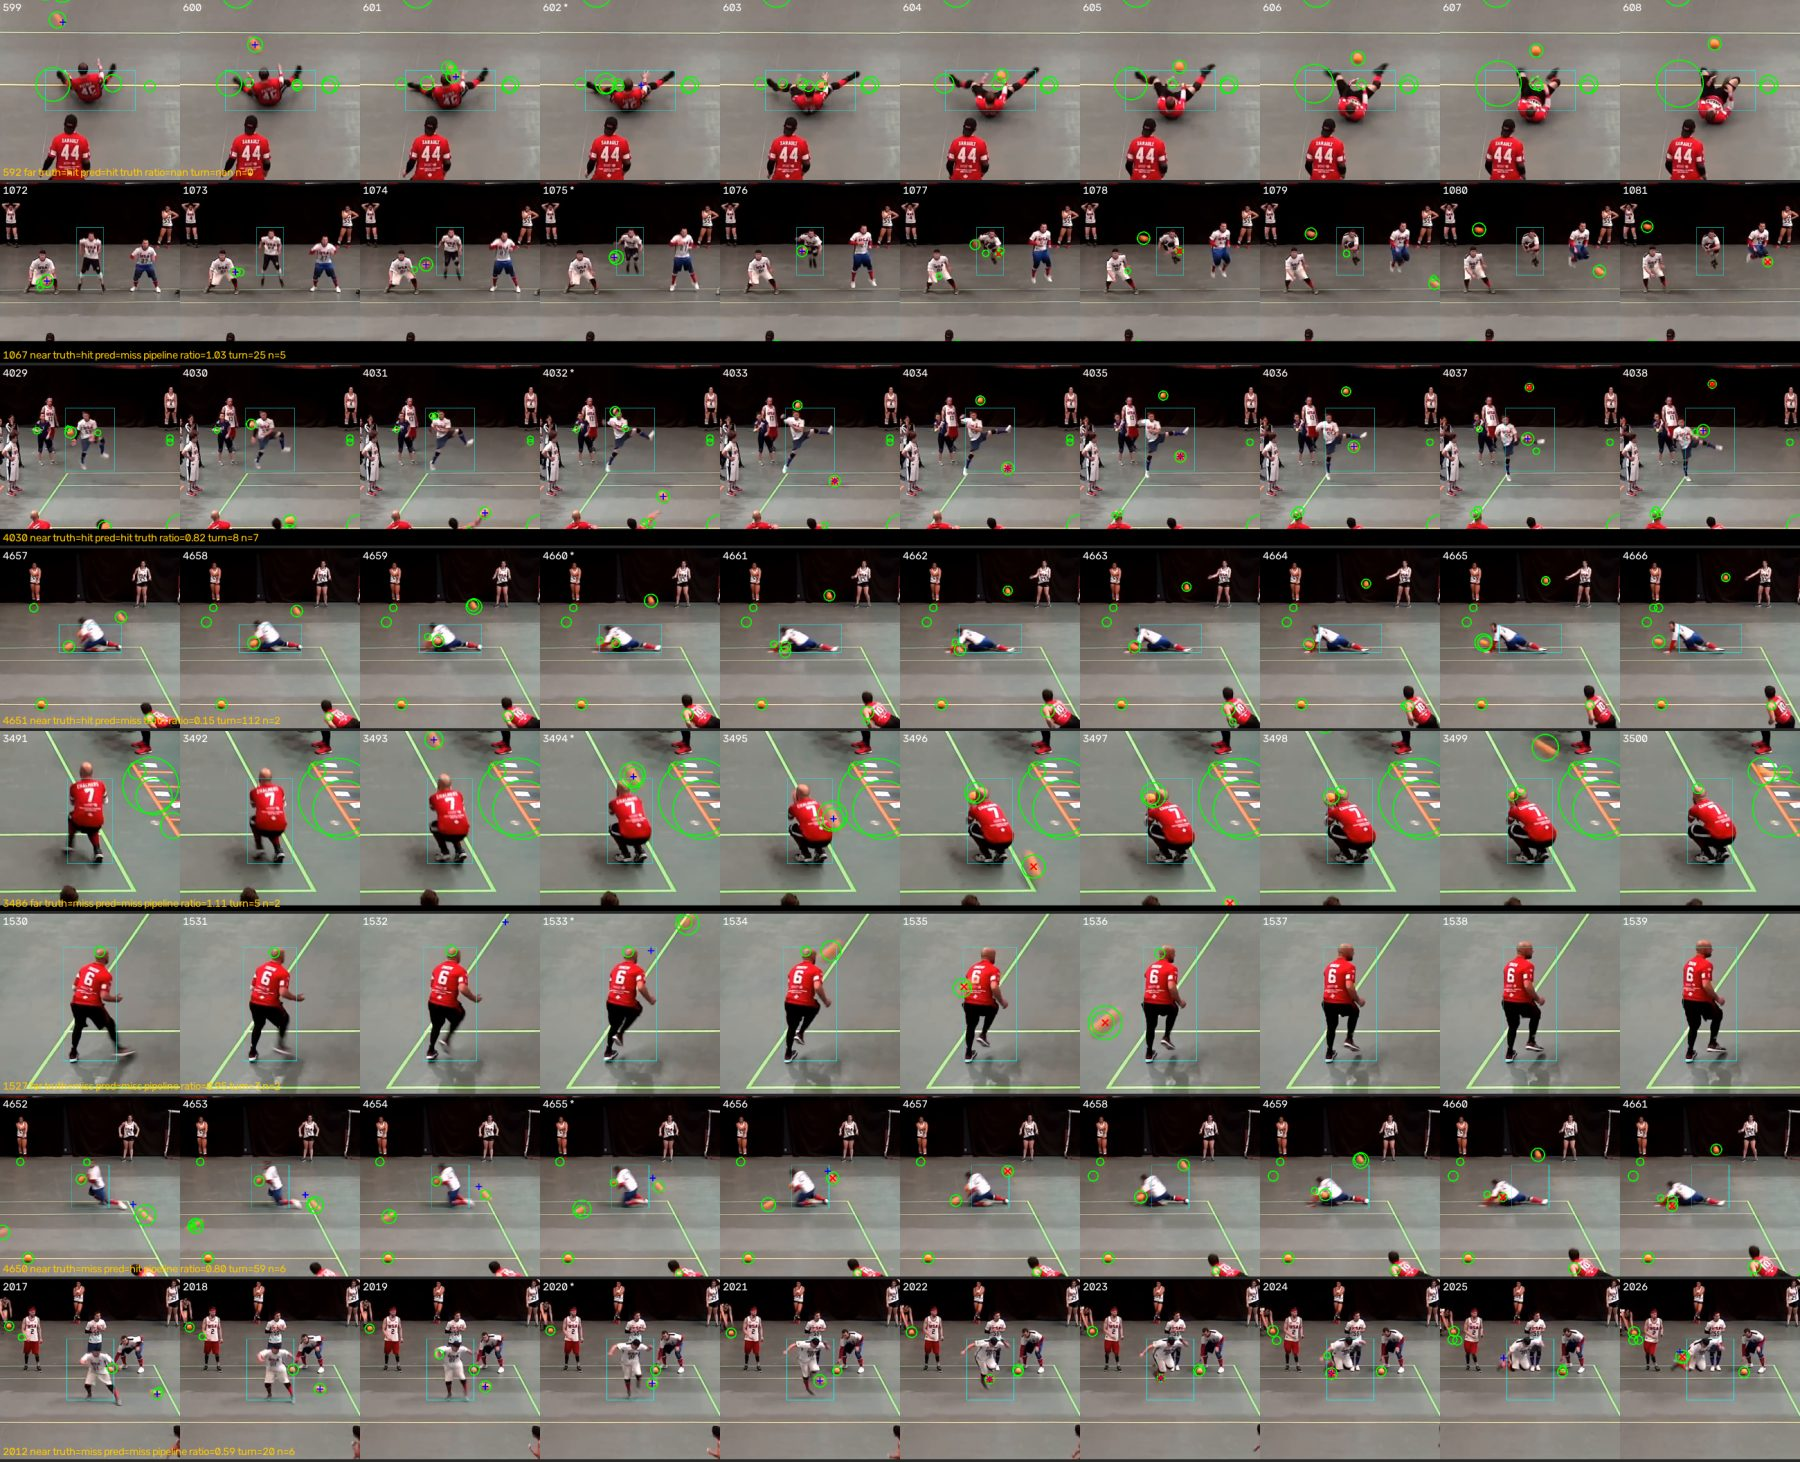
\includegraphics[width=0.92\textwidth]{figures/rebound-hits-v-misses.jpg}
\caption{Four hits above four misses, $\pm$3 frames around the contact. The struck ball
comes back off the player; the missed one carries on past. The turn angle is the one
threshold the rebound stage has.}
\label{fig:rebound}
\end{figure}

\subsection{Audio at the set start only; the body cannot see a release}
\label{sub:signals}

\design{Audio, the whistle band, for set start and outcome corroboration, with a
vision-only against vision-plus-whistle ablation. Pose at and after the peak (follow-through,
arm extension, speed decay) to be tested for feint against throw.}

I thought the whistle would be richer. Referees whistle for eliminations, line violations
and timeouts throughout a set, and the crowd and the shoes are in the same band. The
2.5--4.5\,kHz band fired 56 times in three minutes at a floor low enough to catch quiet
calls, on pump fakes as often as throws; the dozen long, loud ones were real calls and
preceded far-side outs by 0.4 to 4\,s, but two of them had no out behind them at all.
Sixteen whistles clear the prominence floor and one of them starts the set; the rush
whistle measured 37\,dB over the room against 31\,dB for the loudest other, which is not a
margin to build on ungated. Heard only while the balls are laid out on the centre line, a
whistle can mean almost nothing else, so audio is used there and nowhere else. The fusion
ablation was not run because at the outcome there was nothing to fuse.

I thought follow-through might work. On the sixty labelled events and forty-five rejections,
every pose feature tried for fake against release (wrist height at the peak, wind-up depth,
arm extension, elbow angle, torso tilt, body speed, speed decay) sat between AUC 0.4 and
0.7; wrist height, at 0.85 on the first twenty samples, fell to 0.69 on a hundred. A fake is
the same motion with the ball kept and nothing about the motion says so. The next cheapest
test, the ball going dark at the hand after the peak, was AUC 0.75 and wrong in two
systematic ways: a ball tucked behind a body turned to the camera goes just as dark, and a
second ball in the other hand keeps the wrist lit through a real release. So the claim is
made only on \emph{seeing the ball leave}, a chain of ball-sized blobs from the hand
outwards, and absence is never evidence.

\subsection{Destination in the image, and by contact}
\label{sub:dest}

\design{Pass or throw from the departure direction in court metres against the centre
line, via the court homography.}

The floor homography cannot place a ball in the air: at shoulder height it projects metres
beyond the hand, and near-team throwers ``stood'' at court $y$ of 11--15\,m by their ball.
The ball's direction in the image is sound, though, because this camera looks along the
court: the opponent is straight up the frame for the near team and straight down for the
far, and a pass to a teammate goes across. Two tests replaced the metres. Where the chain
reaches a player's box, the rule's own question is asked of that box, which needs no
projection: a teammate is a pass, an opponent a throw. Eighteen of the 30 chained
releases on the clip end in a box, four in a teammate's and fourteen in an opponent's, none
the other way round. Where the chain ends in nobody, the angle between its first links and
the court axis decides; the first links, because the chain's end is whatever the ball
bounced off.

\subsection{Planned and not done}
\label{sub:notdone}

\textbf{Per-event confidence.} Every decision in the cascade is a threshold on a named
quantity and that quantity is written to the timeline (ball mass at the wrist, departure
distance, chain length, turn angle, how long the count step held), so a threshold sweep
reads the file rather than the footage. The mapping from those margins to a $[0,1]$ per
level was not built inside the budget.

\textbf{The blind second labelling pass.} One annotator labelled the clip; the twenty-event
double-label subset the design called for was not run. The label term of the error budget
rests on the annotator's own flags and on the game-state fold instead (\S\ref{sec:budget}),
and the ``what a second annotator would place'' reading of the $\pm$0.25\,s tolerance is
untested.

%=====================================================================
\section{Results}
\label{sec:results}

\texttt{scripts/evaluate.py} scores the timeline one level at a time against the 60
labelled events (25 fakes, 6 passes, 29 throws) at $\pm$6 frames (0.24\,s) and IoU
$\geq$ 0.5 on the thrower's box, matched same-frame same-player through the roster.

{\footnotesize
\begin{xltabular}{\textwidth}{L{40mm} L{54mm} X}
\toprule
\textbf{Level} & \textbf{Score} & \textbf{On}\\
\midrule
Candidate, a throwing motion here & P 84\%\ \ R 93\%\ \ F1 88\% & 67 predictions against 60 events: 56 tp, 11 fp, 4 fn\\
Release frame & MAE 1.1 frames, 44/56 within 2 & matched events\\
Team & 100\% & 56 matched\\
Release, fake against released & 88\% & 56 matched: fakes right 21/23, releases right 28/33\\
Kind, fake / pass / throw & 86\% & 56 matched\\
Throw detection, throw claimed as positive & P 73\%\ \ R 76\%\ \ F1 75\% & 29 truth throws\\
Outcome, hit / catch / block / miss & 82\% & 22 matched throws; 59\% by the count alone\\
Efficiency & near 5/17 = 29\% (truth 4/15 = 27\%)\newline far 1/13 = 8\% (truth 2/14 = 14\%) & per team\\
\bottomrule
\end{xltabular}}

{\footnotesize
\begin{xltabular}{\textwidth}{L{26mm} R{10mm} R{10mm} R{10mm} L{4mm} L{26mm} R{9mm} R{9mm} R{9mm} R{9mm}}
\toprule
\textbf{Kind, truth $\downarrow$} & fake & pass & throw & & \textbf{Outcome, truth $\downarrow$} & hit & catch & block & miss\\
\midrule
fake (23) & \textbf{21} & 2 & 0 & & hit (6) & \textbf{5} & 0 & 0 & 1\\
pass (6) & 1 & \textbf{5} & 0 & & catch (1) & 0 & \textbf{0} & 0 & 1\\
throw (27) & 4 & 1 & \textbf{22} & & block (3) & 0 & 0 & \textbf{2} & 1\\
 & & & & & miss (12) & 1 & 0 & 0 & \textbf{11}\\
\bottomrule
\end{xltabular}}

The timeline is \texttt{data/timeline/wdbf2014\_final\_h2\_set2.json}: every proposal
with frame, team, participant, box, \texttt{released}, \texttt{kind}, \texttt{outcome} and
the evidence behind each claim (ball mass before the peak, departure distance, chain length
and path, contact, turn angle, the count step that resolved the outcome). Dropped
proposals carry why. Detection by kind, with each kind as the positive class: fake F1 78\%,
pass 71\%, throw 75\%.

%=====================================================================
\section{What went wrong}
\label{sec:wrong}

\textbf{Candidate misses (4).} A throw whose wind-up peak landed twelve frames after the
labelled release (the annotator's note calls it late); the two fakes made with no ball,
which the ball gate drops before anything is measured and the harness reports apart; and a throw at 1:49
whose label sits on a second, empty detection of the thrower, so the real thrower's
proposal, with a textbook departure, counts as a false positive against it. That one is the
identity layer's.

\textbf{Candidate false positives (11).} Three are the follow-through of a motion already
matched, twelve to fifteen frames on: the $\pm$6 tolerance splits a wind-up peak from a
release peak. One is the wrong-track thrower above. The rest are a ball wound up and not
thrown at a moment the annotator did not call a fake: a crouch to dodge with the ball
raised, a blocking arm past the line. The loose proposer was doing its job and the
annotator's negatives are unlabelled.

\textbf{Releases called fake (5).} A far-court throw whose ball moved under a diameter a
frame; a throw noted \emph{hard to see} whose ball the mask never got at the hand; a
hand-over the annotator was unsure was a pass; a throw a hair under the departure floor
(0.22 of the scale against 0.25); and the far hit at the set's end, released in a scrum and
never seen leaving. None is a threshold away. \textbf{Fakes called released (2)}, both read
as passes: a ball that split into two colour components in the fingers at the whip, one of
which seeded a chain; and a fake that turned into a hand-off to a teammate. Two more kind
errors, a hard throw that reached a teammate's box first (throw read as pass) and a pass
that left the hand too slowly for the chain (pass read as fake), complete the 8 of 56.

\textbf{Outcome (18 of 22 right; 13 by the count alone).} The rebound witness took five
of the count's nine errors: at 0:43, two near throws ten frames apart with one far
departure, split by the ball that turned (77$^\circ$) against the one that passed straight
through; the blocks at 0:58 and 1:16, turns of 118$^\circ$ and 129$^\circ$ with no count
step behind them, now claimed as \texttt{block}; and 1:48, a hit on a player already out,
which the far departure at 1:56 falls back to once the two spurious near throws after it
are seen to carry on. The four left are three shapes, all in the attribution and none in
the detection, since every count step on the clip is explained by some throw:

\begin{itemize}
\item \emph{The set-ending double}, 3:06. Two near throws a frame apart, a miss then a
hit, whose balls both go through the same far player. The rebound follows both and reads
6$^\circ$ and 34$^\circ$, a graze under its threshold, so recency keeps the later one and
scores two errors.
\item \emph{A return the roster never saw}, 1:47. Two far catches (1:47, 1:49) put two far
players off and the count shows both departures (1:53, 1:56), but only one near player
walking back on (1:58). The second departure has no return to pair with and falls through
to a hit on the latest near throw, a held-ball false positive at 1:50, so the catch scores
miss and near efficiency gains a hit that never happened. Nothing downstream can recover
it.
\item \emph{A block the ball did not show}, 2:09. The third block's track dies inside the
player's box before any turn is seen.
\end{itemize}

The count witness's blind spots are now the graze and the roster's.

%=====================================================================
\section{Error budget}
\label{sec:budget}

\texttt{scripts/error\_budget.py} reads the same matching per team and separates the
model's error from the labels'.

{\footnotesize
\begin{xltabular}{\textwidth}{L{58mm} X X}
\toprule
 & \textbf{near (Canada)} & \textbf{far (USA)}\\
\midrule
Truth efficiency & 4/15 = 27\% & 2/14 = 14\%\\
Predicted & 5/17 = 29\% & 1/13 = 8\%\\
Denominator: throws claimed & 12 true, 5 matched no event, 0 fakes, 0 passes & 10 true, 3 matched no event\\
Denominator: true throws not claimed & 3 (1 called fake, 1 pass, 1 no proposal) & 4 (3 called fake, 1 no proposal)\\
Numerator: hits & 3 right, 1 missed, 2 invented & 1 right, 1 missed, 0 invented\\
\textbf{Model}: paired bootstrap, 95\% band on predicted minus truth & $-$23 to $+$27 points & $-$23 to $+$3 points\\
\textbf{Labels}: every \texttt{uncertain} event decided the other way & 25\% to 33\% & 13\% to 14\%\\
\textbf{Sampling}: Wilson 95\% on the truth itself & 11\% to 52\% & 4\% to 40\%\\
\bottomrule
\end{xltabular}}

Two readings. The near number is right for the wrong reasons: five spurious throws in the
denominator and two invented hits in the numerator cancel to within two points. And the
clip's own sampling interval is wider than any pipeline error: with fifteen throws a side,
this set's efficiency says little about the team's. The metric needs a match rather than a
set, and the pipeline exists so that a match can be scored (\S\ref{sec:scale}).

Label uncertainty was small by the annotator's own flags (three events) but two unflagged
notes mattered more: the throw at 0:58 ``could be a super narrow miss or a hit'' and the
one at 0:59 ``could be block or catch''. Both were decided by folding the labels against
the on-court count, which also found a hit at 1:48 on a player already out (recorded with
\texttt{eliminated: false}, WDBF rule 19.1)\footnote{World Dodgeball Federation, \emph{WDBF
Dodgeball Rules 2024} (2024),
$<$\url{https://worlddodgeballfederation.com/wdbf-content/uploads/2024/03/WDBF-Dodgeball-Rules-2024.pdf}$>$,
accessed 27 August 2026. Quoted by rule number in \texttt{docs/reference/wdbf-rules.md}.}
and turned 0:59 from catch to block because no count moved. The fold is a second annotator
that cannot see the ball.

%=====================================================================
\section{Stress}
\label{sec:stress}

\texttt{scripts/stress.py 480p crf40 drop2}: every pixel-reading stage rerun on a degraded
copy of the clip; the court homography, set boundaries and labels carried over as
deterministic transforms of the source (scaled, or remapped to the kept frames). Tolerance
stays $\pm$0.25\,s.

{\footnotesize
\begin{xltabular}{\textwidth}{L{14mm} L{30mm} R{11mm} R{11mm} R{9mm} R{12mm} R{11mm} R{13mm} L{22mm}}
\toprule
\textbf{Condition} & \textbf{Clip} & \textbf{Cand.\ F1} & \textbf{Release} & \textbf{Kind} & \textbf{Outcome} & \textbf{Throw F1} & \textbf{Pose-only recall} & \textbf{Efficiency near / far}\\
\midrule
source & 1080p, CRF 16, 25\,fps & 88\% & 88\% & 86\% & 82\% & 75\% & 98\% & 29\% / 8\%\\
480p & 854$\times$480, same CRF & 66\% & 90\% & 82\% & 47\% & 67\% & 88\% & 25\% / 20\%\\
crf40 & 1080p, x264 CRF 40 & 51\% & 76\% & 76\% & 67\% & 55\% & 72\% & 38\% / 14\%\\
drop2 & every second frame, 12.5\,fps & 60\% & 93\% & 85\% & 50\% & 64\% & 57\% & 22\% / 8\%\\
\bottomrule
\end{xltabular}}

Truth efficiency is 27\% / 14\% in every row. Release, kind and outcome are on matched
events, whose number falls with candidate recall. The conditions were chosen to break three
different things, and they did.

\textbf{Frame drop looked like a units bug and was not.} The release chain barely noticed
half the frames (release 93\%, kind 85\% on matched events); the loss was at the wind-up
detector, whose windows were frame counts and whose wrist-speed score was displacement per
frame. Restating every window as a duration and the speed as per-second, which is how the
pipeline is now written and changes nothing at 25\,fps, did not recover it: pose-only recall
went from 78\% to 57\%. A throw's whip lasts under 100\,ms, so at 12.5\,fps the peak is
under-sampled and no rescaling of a per-frame score reproduces the 25\,fps threshold. The
detector's sensitivity is a property of the frame rate it was tuned at; a second rate needs
its own score floor, or a detector that models the motion rather than thresholds a peak.

\textbf{480p broke the ball and identity.} Pose still proposed 88\% of the events, but the
ball at the wrists was dropped twice as often (34 ``no ball in hand'' against 20; an 8\,px
ball is a few pixels of hue), the roster fragmented, and the on-court count picked up nine
steps no throw explains (none at source), which took the outcome from 82\% to 47\%, three
misses read as catches off phantom returns. The rebound held up better than the count: the
ball was still followed at 8\,px and two of the three blocks were still seen.

\textbf{Heavy compression broke pose itself.} Blocking artefacts fired the wrist-speed
detector, 137 proposals at 31\% precision, and pose found 72\% of the events.
The gates then worked on what they were given (76\% release, 76\% kind, outcome 67\% on
the dozen throws that survived) but the denominator collapsed, near 8 throws against 15
and far 7 against 14, and the efficiency that came out is a number on half the throws.
CRF 40 is past the cliff; where the cliff is between 16 and 40 was not measured.

The identity layer is rerun in every cell, so a cell's outcome number is partly the
roster's; a mode that carries the source roster across would separate the cascade's limits
from identity's.

%=====================================================================
\section{Ablation}
\label{sec:ablation}

\texttt{scripts/ablate.py}: one pipeline run scored three times with the later stages
withheld. The candidate matching is identical in every row; what moves is what each stage
claims about the same motion.

{\footnotesize
\begin{xltabular}{\textwidth}{L{20mm} L{36mm} R{16mm} R{9mm} R{9mm} R{9mm} R{9mm} R{9mm} R{9mm}}
\toprule
\textbf{Stage} & \textbf{Claims} & \textbf{Predictions} & \textbf{Throw P} & \textbf{Throw R} & \textbf{Throw F1} & \textbf{Fake F1} & \textbf{Pass F1} & \textbf{Kind}\\
\midrule
pose only & wind-up from pose; every proposal a throw & 100 & 28\% & 97\% & 43\% & 0\% & 0\% & 47\%\\
$+$ release gate & ball in hand, ball seen leaving; released means throw & 67 & 61\% & 79\% & 69\% & 78\% & 0\% & 79\%\\
$+$ destination & pass or throw & 67 & 73\% & 76\% & 75\% & 78\% & 71\% & 86\%\\
\bottomrule
\end{xltabular}}

The release gate was worth 33 points of throw precision and cost 18 of recall, the five
releases it calls fake. The destination test bought 12 more points of precision for 3 of
recall, and is the only stage that finds a pass. The pose-only row is the simple
baseline the brief asks for: a single-signal detector that calls every motion a throw is
43\% F1 on throws and cannot see a fake or a pass.

%=====================================================================
\section{The metric at scale}
\label{sec:scale}

The metric's natural follow-up is whether \emph{how} a throw is set up changes whether it
converts. Two splits the timeline supports (\texttt{scripts/tactics.py}):
\textbf{coordinated}, an \emph{attack} of two or more same-team throws released within
300\,ms, the tactic against a lone dodger who can only dodge one ball; and
\textbf{fake-led}, same-team fakes in the 6\,s before a throw. Coordination is scored per
attack rather than per throw: two balls for one out is the tactic working, and per throw it
would read as one for two. On the labelled set the bins hold one and two events, so the
whole second half (23 minutes, eight sets, no labels) was run through the pipeline to see
what holds over 240 predicted throws.

{\footnotesize
\begin{xltabular}{\textwidth}{L{30mm} L{8mm} L{18mm} L{18mm} L{18mm} L{16mm} L{13mm} L{13mm}}
\toprule
 & \textbf{Team} & \textbf{All throws} & \textbf{Solo attacks} & \textbf{Coordinated} & \textbf{Fakes before: 0} & \textbf{1} & \textbf{2$+$}\\
\midrule
labelled set, truth & far & 2/14 = 14\% & 2/12 = 17\% & 0/1 & 2/9 = 22\% & 0/3 & 0/2\\
labelled set, truth & near & 4/15 = 27\% & 3/13 = 23\% & 1/1 & 2/5 = 40\% & 2/8 = 25\% & 0/2\\
same set, predicted from the half & far & 2/11 = 18\% & 2/11 = 18\% & --- & 0/3 & 1/2 & 1/6\\
same set, predicted from the half & near & 5/18 = 28\% & 4/13 = 31\% & 1/2 & 3/11 = 27\% & 2/4 & 0/3\\
\textbf{whole half, predicted} & far & \textbf{47/114 = 41\%} & 43/104 = 41\% & 4/5 = 80\% & 25/66 = 38\% & 17/32 = 53\% & 5/16 = 31\%\\
\textbf{whole half, predicted} & near & \textbf{23/126 = 18\%} & 21/101 = 21\% & 2/11 = 18\% & 14/65 = 22\% & 6/42 = 14\% & 3/19 = 16\%\\
\bottomrule
\end{xltabular}}

Three readings, all with the outcome level's 82\% attached.

\begin{itemize}
\item \textbf{The pipeline reproduced itself across cuts.} The labelled set scored from the
whole-half run (set 3 of 8) landed where the clip run did: near 28\% against 27\% truth,
far 18\% against 14\%. Set boundaries, roster and outcomes were all re-derived from 23
minutes of footage with no labels involved.
\item \textbf{USA converted twice as often as Canada across the half}, 41\% against 18\%,
and seven of the eight sets have the far side ahead. That is the match-level statement the
metric exists to make, and it is not visible in one set.
\item \textbf{Coordinated attacks: 4 of 5 far, 2 of 11 near}, against solo rates of 41\%
and 21\%. The one coordinated attack in the truth set is the set-ending double on the last
player standing, the situation the tactic exists for; five and eleven attacks cannot separate a
tactic from noise (the far figure was 2 of 5 before the rebound stage moved two outcomes),
and the half says only that the question is askable. Fake-led throws showed no consistent
direction.
\end{itemize}

The half also showed the pipeline's limits at scale: 36 count steps no throw explains
(eliminations whose throw the cascade missed or called fake), and identity fragmenting over
1,402 tracks, with the far team's numbers read on some sets and not others, which the
outcome fold survives because it counts bodies, not names.

%=====================================================================
\section{What the numbers cannot say}
\label{sec:uncertain}

\begin{itemize}
\item \textbf{Recall is measured against a truth set the candidate stage seeded.} Every
event was labelled from a proposal (accept, reject or adjust), so candidate recall would be
1.0 by construction unless proposals were missed; the stage was built loose for that reason
(100 proposals for 60 events), and the number is better read as the precision of a
recall-tuned stage. One annotator; the blind second pass was not run
(\S\ref{sub:notdone}).
\item \textbf{The ball is colour.} An HSV mask with a hue floor one step above the red
jersey, ball-sized components only. It cannot see a ball against the red team at the far
baseline, and it cannot tell one ball from another when two cross; the rules that untangle a
crossing are geometric.
\item \textbf{The outcome is the count's, with the ball as witness.} A count step is
attributed to the last throw at that side unless a ball was seen to turn at a player; a turn
nobody left for is a block. The rebound's one threshold was set by eye on the clip it is
scored on, from six visible hits, and a graze under it reads as a pass-through.
\texttt{catch} is the count's alone.
\item \textbf{Identity is one clip deep.} Seven players named of twelve; the far team is
largely unnamed, its numbers unreadable at 90\,px. Attribution is by track and side, which
is what the metric needs; player-level attribution is reported where the number is known and
no further.
\item \textbf{One camera, one venue.} The court fit, the ball colour and the kit rules are
all this footage's. Nothing here has seen a second venue.
\end{itemize}

%=====================================================================
\section{Ground truth}
\label{sec:truth}

{\footnotesize
\begin{xltabular}{\textwidth}{L{24mm} X}
\toprule
\textbf{Amount} & One clip, 3.5\,min, one complete set; 60 closed events: 25 fakes (2 with no ball), 6 passes, 29 throws (7 hits, 2 catches, 5 blocks, 15 misses); 105 proposal reviews, 18 with notes\\
\textbf{Rule} & \texttt{docs/labeling-guide.md}, written to be handed to a second person. Anchor on the release frame; thrower clicked at release, target at the end; team from the court half; \texttt{kind} by destination; ambiguous cases flagged \texttt{uncertain} with a note; \texttt{release\_visible}, \texttt{outcome\_visible} and \texttt{ref\_signal} recorded so label uncertainty is separable from model error\\
\textbf{Where it is uncertain} & Three flagged events (a very close miss, a hand-over that may be a pass, a fake that became a dodge); two notes on unflagged events (0:58 hit or miss, 0:59 block or catch); two labels corrected by the game-state fold (0:59 catch to block, 1:48 hit with \texttt{eliminated: false}), each with the reason in its note\\
\textbf{Storage} & Boxes are stored by value in source pixels, never as track ids, so the truth survives a change of detector. Every label file records the clip hash\\
\textbf{Tool} & \texttt{tools/labeler/}: proposals shown as rings, one keypress to accept, reject or classify, player keys mapped through the roster, every box snapped to the same pose run the pipeline reads\\
\bottomrule
\end{xltabular}}

The design estimated 50 to 70 throws and 10 to 20 feints in a set; the set held 29 throws,
6 passes and 25 fakes. Fakes were twice as common as planned for and passes rarer, which is
why the pass column carries the widest interval of any level.

%=====================================================================
\section{Compute, measured}
\label{sec:compute}

Batch. One laptop RTX 4080 at an 80\,W cap; the whole clip in about twelve minutes, of
which pose is ten.

{\footnotesize
\begin{xltabular}{\textwidth}{L{40mm} L{30mm} X}
\toprule
\textbf{Stage} & \textbf{Measured, 3.5\,min clip} & \textbf{Note}\\
\midrule
Pose, YOLO11x-pose at 1920\,px, single precision & 9.0--9.4\,fps, 10\,min & The design budgeted 5\,min at half precision (table below); the pipeline ran single precision\\
Court fit & seconds & once per clip\\
Identity: tracking and OCR & 24\,s & over precomputed detections\\
Set start, set end & seconds & \\
Candidates & 3\,s & arithmetic over the pose run\\
Release gate & 52\,s & one sequential decode of the clip around every proposal\\
Rebound & $\sim$3\,s per throw that reached a player & SAM~2 large on a moving crop, a model load per segment\\
Evaluation, error budget & 1\,s & \\
\midrule
\textbf{Training} & none & \\
\bottomrule
\end{xltabular}}

Half precision was benchmarked on 250 frames of the clip after the results were frozen:

{\footnotesize
\begin{xltabular}{\textwidth}{L{50mm} L{20mm} X}
\toprule
\textbf{Setting} & \textbf{fps} & \textbf{Keypoints against single precision}\\
\midrule
FP32, one frame at a time (as run) & 9.0--9.4 & \\
FP16, one frame at a time & 18.0 & median 0.43\,px, p95 0.56\,px; 4 of 9,256 detections differ\\
FP16, batch of 8 & 7.3 & same as FP16\\
FP32, batch of 8 & 6.8, out-of-memory warning at 5.7\,GiB & median 0.02\,px\\
\bottomrule
\end{xltabular}}

Half precision doubles throughput for a sub-pixel change in keypoints, and the design's
budget assumes it. Batching is slower: one 1920\,px frame already saturates this GPU,
and batching adds memory and CPU preprocessing. The first run of the day reads about
5\,fps because the GPU idles at 210\,MHz until warm.

%=====================================================================
\section{Next experiment}
\label{sec:next}

Score the rebound witness blind. It was built, and its one threshold set, on the clip it
is scored on, from six visible hits (figure~\ref{fig:rebound}); the second set of the half
is where it holds or does not. Three things to read off that run. Whether the turn
threshold holds: the set's last hit is a 34$^\circ$ graze that reads as a pass-through, and
a second set says whether grazes are the exception. The tracks that die inside a box (the
block at 2:09, which has no answer): the tracker loses a ball that drops straight down behind
a body, and a second segment seeded on the colour mask at the feet is the patch to try. And
the fast far-side throws where the tracker leaves the ball before it arrives: an optical-flow
bridge across the lost frames from the last good position, which cost nothing on this clip
and will on a faster one.

\textbf{Further out.} A second venue should cost a config change and a retune: the
colour window, court dimensions and kit vocabulary are in \texttt{config/venue.toml}, the
court fit checks itself against markings it did not fit to, and every input is keyed to the
clip's hash, so the pipeline fails loudly at a new venue rather than adapting to it, which is
the right first failure. A learned ball detector is the next model and was not
built: the event needs the ball only at the thrower's wrists and along its first metre of
flight, which colour gives at this camera, and six identical balls in constant hand-off
would make global tracking a linking problem needing fine-tuning and association work that
the release gate does not need. It becomes worth it when the colour mask is the limit: the
far baseline at 480p, or a venue whose kit shares the ball's hue.

%=====================================================================
\section{Reproducing}
\label{sec:repro}

Python 3.12, \texttt{ffmpeg}, \texttt{ffprobe} and \texttt{yt-dlp} on PATH, a CUDA GPU
for pose (CPU works, slowly). Footage and pose runs are never committed; labels, court fit,
set boundaries, roster, candidates and the timeline are.

{\footnotesize
\begin{verbatim}
python -m venv .venv && .venv/bin/pip install -r requirements.txt
.venv/bin/python scripts/download_weights.py          # yolo11x-pose (~113 MB), sam2_l (~224 MB)
scripts/download_footage.sh && scripts/make_clip.sh   # WDBF 2014 final, 2nd half -> 6:00-9:30 clip
.venv/bin/python scripts/run.py data/footage/wdbf2014_final_h2_set2.mp4 --offset 360
make evaluate   # every level            make budget    # error budget
make stress     # the three conditions   make ablate    # the cascade withheld stage by stage
make tactics    # the set-up split       make test      # every suite
\end{verbatim}}

%=====================================================================
\section{Assistance and sources}
\label{sec:sources}

Claude Code was used throughout as a pair: drafting modules and tests against a plan
agreed first, running the evaluations, and writing the architecture docs as each stage
shipped. Every design decision was taken in conversation and is recorded with its
rationale in \texttt{docs/}; every label was placed by hand, and both documents were written
by me with the assistant as editor.

\section*{Bibliography}
\addcontentsline{toc}{section}{Bibliography}

\raggedright\sloppy
\begin{itemize}[leftmargin=1.4em,label={},itemsep=4pt]
\item Baek, Y., Lee, B., Han, D., Yun, S. and Lee, H., `Character Region Awareness for
Text Detection', in \emph{2019 IEEE/CVF Conference on Computer Vision and Pattern
Recognition} (Long Beach, 2019), pp.\ 9357--9366.
\item JaidedAI, \emph{EasyOCR} (version 1.7), software,
$<$\url{https://github.com/JaidedAI/EasyOCR}$>$, accessed 27 August 2026.
\item Jocher, G., Qiu, J. and Chaurasia, A., \emph{Ultralytics YOLO} (version 8.4),
software, 2024, $<$\url{https://github.com/ultralytics/ultralytics}$>$, accessed
27 August 2026.
\item Ravi, N., Gabeur, V., Hu, Y.-T., Hu, R., Ryali, C., Ma, T., Khedr, H., R\"adle, R.,
Rolland, C., Gustafson, L., Mintun, E., Pan, J., Alwala, K.\ V., Carion, N., Wu, C.-Y.,
Girshick, R., Doll\'ar, P. and Feichtenhofer, C., `SAM 2: Segment Anything in Images and
Videos', arXiv:2408.00714, 2024, $<$\url{https://arxiv.org/abs/2408.00714}$>$, accessed
27 August 2026.
\item World Dodgeball Federation, \emph{2014 World Dodgeball Championship, Men's Final:
Canada v USA} [video], YouTube, $<$\url{https://www.youtube.com/watch?v=Spu6OlAZHUo}$>$,
accessed 27 August 2026.
\item World Dodgeball Federation, \emph{WDBF Dodgeball Rules 2024} (2024),
$<$\url{https://worlddodgeballfederation.com/wdbf-content/uploads/2024/03/WDBF-Dodgeball-Rules-2024.pdf}$>$,
accessed 27 August 2026.
\item Zhang, Y., Sun, P., Jiang, Y., Yu, D., Weng, F., Yuan, Z., Luo, P., Liu, W. and
Wang, X., `ByteTrack: Multi-Object Tracking by Associating Every Detection Box', in
\emph{Computer Vision -- ECCV 2022}, Lecture Notes in Computer Science 13682 (Cham:
Springer, 2022), pp.\ 1--21.
\end{itemize}

\end{document}
